\chapter{Recolección de Datos}\label{chap:recoleccion}

En este capítulo veremos las diferentes imágenes que se utilizaron para el desarrollo de la tesis; se expondrá además, las diversas configuraciones utilizadas para la realización de los experimentos y los diferentes pasos que se siguió para la recolección de las imágenes.


\section{Imágenes Satelitales}\label{sec:imagen_satelitales}

Una imagen satelital se la puede definir como la representación visual de información capturada por un sensor montado en un satélite artificial. Estos sensores recogen la información reflejada por la superficie de la tierra que luego es enviada para su posterior procesamiento.

El uso de imágenes satelitales constituye una excelente herramienta para el conocimiento y monitoreo de los territorios y recursos; hoy en día disfrutamos de la oportunidad de aprovechar de imágenes satelitales para una gran variedad de aplicaciones:
\begin{itemize}
	\item Desarrollo y planificación urbana.
	\item Infraestructura, carreteras, canales, tuberías etc.
	\item Recursos naturales.
	\item Investigación.
	\item Alerta temprana de catástrofes.
	\item Asuntos militares.
	\item entre otras aplicaciones.
\end{itemize}

\subsection{Niveles de procesamiento}\label{sub:nivelesdeprocesamiento}
Dependiendo de la agencia espacial existe una nomeclatura para determinar los niveles de procesamiento que se aplica a las imágenes satelitales. En nuestro caso vamos a utilizar las siguientes:
\begin{itemize}
	\item \textbf{Nivel 0}: La información científica recogida está a máxima resolución, ordenada temporalmente y con errores de transmisión, artefactos y duplicados eliminados.
 	\item \textbf{Nivel 1a}: La información esta ordenada cronológicamente y datos auxiliares como coeficientes de calibración y parámetros de referencia.
 	\item \textbf{Nivel 1b}: La información del 1a es procesada a unidades de detección, georefereciada.
 	\item \textbf{Nivel 2}: Variables geofísicas derivadas por ejemplo productos de concentraciones de hielo, ola de mar, etc.
 	\item \textbf{Nivel 3}: Las variables son mapeadas uniformemente en \textit{grids} espacio-temporales.
 	\item \textbf{Nivel 4}: Resultados de los análisis de los niveles anteriores
\end{itemize}


\subsection{Imágenes utilizadas}\label{sub:datosutilizados}
Los datos utilizados para la realización de esta tesis fueron extraidos a través del catálogo de imágenes publicadas en la web oficial, \ac{conae} \footnote{Fuente: http://catalogos.conae.gov.ar/catalogo/catalogo-de-imagenes.html}. Las imágenes que se obtuvieron son de naturaleza óptica pertenecientes al satélite Suomi-NPP, tomadas por el instrumento \ac{viirs} \ref{sub:viirs}.

Como se mencionó en la sección \ref{sec:funcamentacion}, las imágenes que se seleccionaron para el desarrollo de la tesis se asemejan a las característica de la cámara a ser utilizada por el proyecto "Formador Saltelital FS2017"  \ac{conae}.

\subsubsection{VIIRS}\label{sub:viirs}
El instrumento \ac{viirs} fue lanzado a bordo del satélite Suomi-NPP el 28 de octubre de 2011. Este instrumento posee 5 canales de alta resolución (I-bands), 16 canales de resolución moderada (M-bands) y un canal de baja luz (Day/Night Band, DNB). 

En el siguiente cuadro se detallan las diferentes lingitudes de onda y los rangos de onda de las bandas, junto con resolución geométrica apuntando a Nadir (ver tabla: \ref{tab:viirs}).
\begin{table}[H]
\begin{center}
\begin{tabular}{|c|c|c|}
\hline Banda & Rango Espectral (um) & Resolución Nadir \\\hline 
 		M1  & 0.402-0.422   & 0.742 x 0.259 \\ \hline 
		M2  & 0.436-0.454   & 0.742 x 0.259 \\ \hline 
		M3  & 0.478-0.498   & 0.742 x 0.259 \\ \hline 
		M4  & 0.545-0.565   & 0.742 x 0.259 \\ \hline 
		I1  & 0.600-0.680   & 0.371 x 0.387 \\ \hline 
		M5  & 0.662-0.682   & 0.742 x 0.259 \\ \hline 
		M6  & 0.739-0.754   & 0.742 x 0.776 \\ \hline 
		I2  & 0.846-0.885   & 0.371 x 0.387 \\ \hline 
		M7  & 0.846-0.885   & 0.742 x 0.259 \\ \hline 
		M8  & 1.230-1.250   & 0.742 x 0.776 \\ \hline 
		M9  & 1.371-1.386   & 0.742 x 0.776 \\ \hline 
		I3  & 1.580-1.640   & 0.371 x 0.387 \\ \hline 
		M10 & 1.580-1.640   & 0.742 x 0.776 \\ \hline 
		M11 & 2.225-2.275   & 0.742 x 0.776 \\ \hline 
		I4  & 3.550-3.930   & 0.371 x 0.387 \\ \hline 
		M12 & 3.660-3.840   & 0.742 x 0.776 \\ \hline 
		M13 & 3.973-4.128   & 0.742 x 0.259 \\ \hline 
		M14 & 8.400-8.700   & 0.742 x 0.776 \\ \hline 
		M15 & 10.263-11.263 & 0.742 x 0.776 \\ \hline 
		I5  & 10.500-12.400 & 0.371 x 0.387 \\ \hline 
		M16 & 11.538-12.488 & 0.742 x 0.776 \\ \hline 
\end{tabular}
\end{center}\caption{Característica de bandas,\ac{viirs} \label{tab:viirs}}
\end{table}

Las bandas  utilizadas para este trabajo de tesis  son las  de resolución moderada (M-bands), que posee una resolución espacial a nadir de 750 metros. Además de selecciónar las bandas para el desarrollo, se trabajó con imágenes correspondiente a los años 2017 y 2018 en una ventana de tiempo desde Abril del 2017 a Marzo del 2018.  Las imágenes satelitales obtenidas son productos con  un nivel de procesamiento \textit{nivel 1b}, ver:\ref{sub:datosutilizados}.  

En la siguiente figura \ref{Fig: bandas543} podemos visualizar las características de las imágenes utilizadas; en este caso una imágen correspondiente a la combinaciónes de bandas M5, M4, M3 llamadas (\textit{True Color}).




\begin{figure}[h]
 \centering
  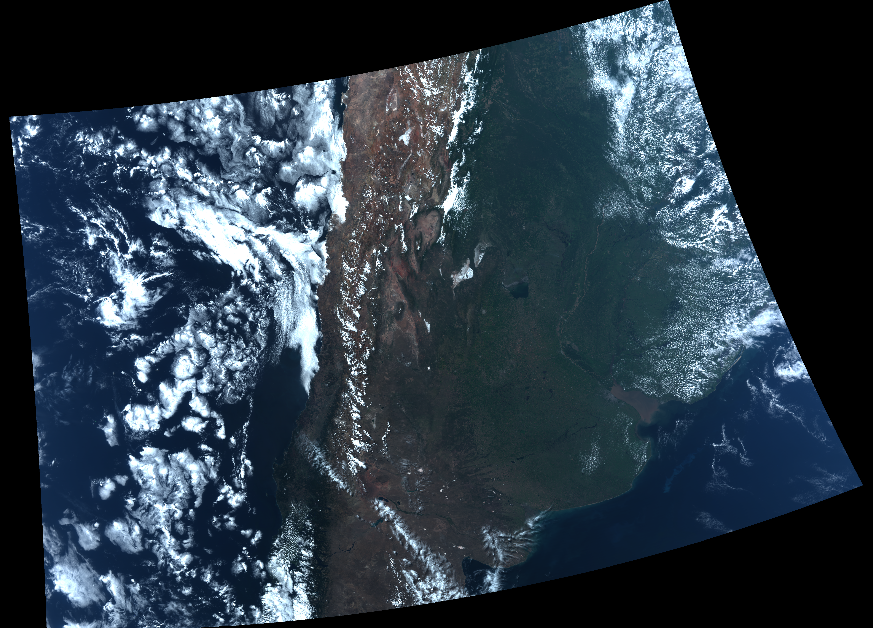
\includegraphics[height=10cm,keepaspectratio=true,clip=true]{imagenes/RecolecciondeDatos/img-543.png}
  \caption{Combinación de bandas M5, M4 y M3, Suomi-NPP}
	\label{Fig: bandas543}
\end{figure}


\section{Obtención de las Imágenes}\label{sub:obtencioimagen}

Para recolectar las imágenes mencionadas en la sección anterior: \ref{sub:datosutilizados}, se debió seguir diversos pasos de las cuales detallamos a continuación:
\begin{enumerate}
	\item Descarga de imágenes del sitio oficial de \ac{conae}.
	\item Pre-procesamiento para obtener una imagen geo-referenciada
\end{enumerate}

Para realizar el pre-procesamiento se utilizo la herramienta ENVI \ref{sub:enviSoft}, software de análisis de imágenes. Este software nos proporciona diferentes herramientas para la manipulación y procesamiento  de  una imagen satelital, de las cuales podemos mencionar la \textit{VIIRS Conversion Toolkit}, esta herramienta nos permite trabajar con productos \ac{viirs}, pudiendo aplicar a las imágenes correcciones geométricas, geo-referenciacion y re-proyecciones entre sus diferentes funcionalidades que nos brinda.

A continuación se detallan los pasos llevados a cabo para la obtención de una imagen por medio de  \textit{ENVI}.
\begin{enumerate}
\item Inicio, pantalla principal ENVI:
	\begin{figure}[h]\centering
 		 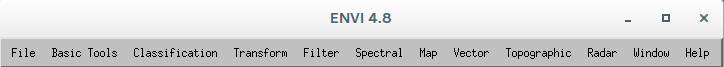
\includegraphics[height=1.5cm,keepaspectratio=true,clip=true]{imagenes/RecolecciondeDatos/envi1.png}
  			\caption{Pantalla Principal ENVI} \label{Fig: envi1}
	\end{figure}


\item Procesamiento: abrir la herramienta \textit{VIIRS Conversion Toolkit} e ingresar los archivos de cada banda adjuntando el archivo de la georeferenciasión, para realizar la carga de la imagen (figura: \ref{Fig: envi2}).

\begin{figure}[h] \centering
  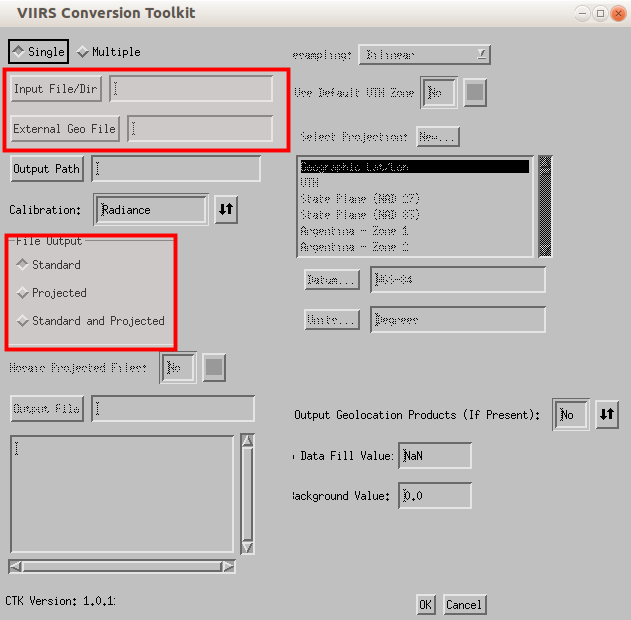
\includegraphics[height=9cm,keepaspectratio=true,clip=true]{imagenes/RecolecciondeDatos/envi2.png}
  \caption{Cargar Bandas ENVI Toolkit} \label{Fig: envi2}
\end{figure}


\item Re-proyección de imagen: adjuntar bandas a utilizar; se debe asignar de acuerdo al color que corresponda cada banda (RGB) (figura: \ref{Fig: envi3}).
 
\begin{figure}[h]
 \centering
  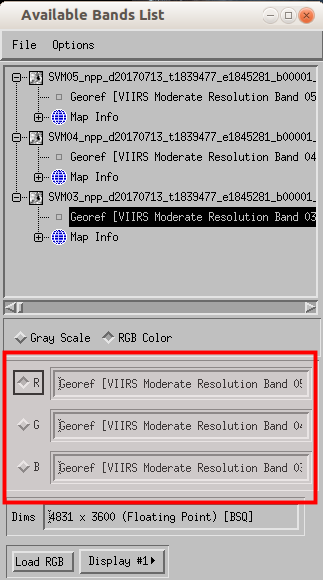
\includegraphics[height=9cm,keepaspectratio=true,clip=true]{imagenes/RecolecciondeDatos/envi3.png}
  \caption{Ejemplo re-proyección \textit{True Color}}
	\label{Fig: envi3}
\end{figure}

\end{enumerate}

Las imágenes obtenidas se almacenaron en una archivo \textit{.tiff}